\section{Additional Experiments}
\label{app:additional_experiments}

This appendix reports supplemental robustness and implementation-fidelity analyses for Section~\ref{sec:experiments}. Section~\ref{app:nested_wait_pseudocode} records the full event-driven Nested WAIT pseudocode used for implementation. Section~\ref{app:no_wait} isolates the role of the accumulation requirement by comparing WAIT with a threshold-only variant. Section~\ref{app:gpu_validation} validates the simulator against direct GPU measurements and reports supplemental physical-GPU comparisons on single-type and real-data workloads. Section~\ref{app:multi_seed} examines repeated-run variability near the observed transition from near-overloaded to overloaded operation, and Section~\ref{app:pd_disagg} evaluates the policy in a prefill-decode-disaggregated deployment.

\subsection{Nested WAIT implementation pseudocode}
\label{app:nested_wait_pseudocode}

Algorithm~\ref{alg:nested_wait_full} gives the event-driven implementation corresponding to the main-text description in Algorithm~\ref{alg:nested_wait}. It makes explicit the queue transitions at segment boundaries and the LIFO memory-repair rule for resident boundary queues.

\begin{breakablealgorithm}
\caption{Full Event-Driven Implementation of Nested WAIT}
\label{alg:nested_wait_full}
{\footnotesize\linespread{0.98}\selectfont
\begin{algorithmic}[1]
\Require Memory capacity \( C \), arrival rates \( \lambda_j \) for \( j \in [m] \), thresholds \( n_k \) for segments \( k \in [m] \)
\Require Output lengths \( l_1' < l_2' < \cdots < l_m' \) for output-length classes \( j \in [m] \)
    \Statex \Comment{$Q_{1,0}$ is external; for $k\ge2$, $Q_{k,l_{k-1}'}$ waits outside segment $k$ but remains GPU-resident}
    \Statex \Comment{Prompts in stages $l_{k-1}'+1,\ldots,l_k'$ have already been admitted into segment $k$}
    \Statex \Comment{Memory repair evicts prompts from resident boundary queues in LIFO order and returns them to $Q_{1,0}$}
    \State Initialize all segment-entry, boundary, and interior queues to zero
    \State Initialize event queue; set current time \( t \gets 0 \)
    \State Set server status to idle
    \While{True}
        \State Wait for the next event (arrival or batch completion)
        \If{event is an arrival}
            \State \( Q_{1,0} \gets Q_{1,0} + 1 \)  \Comment{New prompts enter segment 1 at stage 0}
        \ElsIf{event is a batch completion for prefix \(1,\dots,k\)}
            \State Retrieve the selected counts \(a_{k's}\) stored with the completed prefix batch
            \State Update all affected queues simultaneously using pre-completion queue values
            \For{each processed segment \( k'\le k \)}
                \For{each selected nonterminal stage \(s<l_{k'}'\)}
                    \State \(Q_{k',s}\gets Q_{k',s}-a_{k's}\), \quad \(Q_{k',s+1}\gets Q_{k',s+1}+a_{k's}\)
                \EndFor
                \If{\(k'<m\)}
                    \State Let \(c_{k'}\) be the number of selected prompts at \(l_{k'}'\) that complete there
                \Else
                    \State Set \(c_m\gets a_{m,l_m'}\)
                \EndIf
                \State Set the survivor count \(r_{k'}\gets a_{k',l_{k'}'}-c_{k'}\)
                \State \(Q_{k',l_{k'}'}\gets Q_{k',l_{k'}'}-a_{k',l_{k'}'}\)
                \If{\(k'<m\)}
                    \State \(Q_{k'+1,l_{k'}'}\gets Q_{k'+1,l_{k'}'}+r_{k'}\) \Comment{Survivors join the next resident boundary queue}
                \Else
                    \State Clear KV caches of completed prompts
                \EndIf
            \EndFor
            \While{\(M_{\mathrm{res}}(Q)>C\) and a resident boundary queue is nonempty}
                \State Choose \(h\ge2\) whose resident boundary queue contains the most recently admitted prompt
                \State \(Q_{h,l_{h-1}'}\gets Q_{h,l_{h-1}'}-1\), \quad \(Q_{1,0}\gets Q_{1,0}+1\)
                \State Discard the evicted prompt's KV cache and accumulated progress
            \EndWhile
            \State Set server status to idle
        \EndIf
        \State Find largest \( k \) such that \( Q_{k', l_{k'-1}'} \geq n_{k'} \) for all \( k' \leq k \) \Comment{All segments up to $k$ meet threshold}
        \If{server is idle and such \( k \) exists}
            \State Set \(S_1=\{0,\ldots,l_1'\}\)
            \State For \(k'=2,\ldots,k\), set \(S_{k'}=\{l_{k'-1}',\ldots,l_{k'}'\}\)
            \State For every \(k'\le k\) and \(s\in S_{k'}\), set \(a_{k's}\gets\min\{n_{k'},Q_{k',s}\}\)
            \State Form the prefix batch from all selected prompts and store \(a_{k's}\)
            \State Let \(Q^+\) be the conservative projected post-iteration queue state
            \While{\(M_{\mathrm{res}}(Q^+)>C\) and an unselected resident boundary prompt exists}
                \State Choose \(h\ge2\) whose unselected resident boundary prompts include the most recently admitted prompt
                \State \(Q_{h,l_{h-1}'}\gets Q_{h,l_{h-1}'}-1\), \quad \(Q_{1,0}\gets Q_{1,0}+1\)
                \State \(Q^+_{h,l_{h-1}'}\gets Q^+_{h,l_{h-1}'}-1\)
                \State Discard the evicted prompt's KV cache and accumulated progress
            \EndWhile
            \State Process batch; already resident prompts outside the batch wait with their KV caches retained
            \State Set server status to busy until the completion event for this prefix batch
        \EndIf
    \EndWhile
\end{algorithmic}
}
\end{breakablealgorithm}


\subsection{Threshold without waiting}
\label{app:no_wait}

We isolate the role of waiting on the single-type \texttt{p512d20} workload by comparing full WAIT with a threshold-only variant, denoted \emph{WAIT-no-wait}. For each arrival rate, the two policies use the same parameter setting and hence the same threshold upper bound. The threshold-only variant enforces this upper bound but does not wait for enough requests to accumulate before service. The comparison therefore holds the admission-capacity scale fixed and changes only whether service is delayed to form a full threshold batch.

Figure~\ref{fig:wait_gate_ablation} reports the comparison across arrival rates. At low arrival rates, waiting introduces a modest latency cost: requests may wait to accumulate even when the server has enough capacity to process them immediately. This cost shrinks as the arrival rate increases. Near the overload boundary, waiting becomes useful because it regulates the timing at which work enters service, reducing latency relative to the threshold-only variant. Once the system is overloaded, the upper bound becomes the dominant control, and the two variants again behave similarly.

\begin{figure}[ht]
    \centering
    
\includegraphics[width=0.78\textwidth]{Experiments_pdf/figure_K_wait_gate_ablation.pdf}
    \caption{Effect of waiting on the single-type \texttt{p512d20} Vidur workload. At each arrival rate, full WAIT and the threshold-only variant use the same parameter setting; the comparison only changes whether service waits for enough requests to accumulate before scheduling.}
    \label{fig:wait_gate_ablation}
\end{figure}

\subsection{Real-GPU validation}
\label{app:gpu_validation}

We complement the Vidur experiments in Section~\ref{sec:experiments} with measurements on a physical NVIDIA A100~80\,GB serving Llama-2-7B. These runs serve two purposes. First, direct GPU measurements calibrate the iteration-time model used by Vidur. Second, we implement WAIT's admission logic using SGLang~0.5.7, an open-source LLM serving framework~\citep{sglang-github}, and test the resulting scheduler in end-to-end GPU runs. We report three comparisons: iteration-time measurements against Vidur's prediction, a single-type GPU workload corresponding to Section~\ref{sec:exp_synthetic}, and a real-data GPU workload corresponding to Section~\ref{sec:exp_real}.

\paragraph{Simulator vs GPU.}
To calibrate the simulator in the operating region used in Section~\ref{sec:experiments}, we compare Vidur's iteration-time predictions with direct measurements on the same A100~80\,GB GPU running Llama-2-7B under the SGLang baseline scheduler. Vidur's raw Llama-2-7B attention profiling covers batch sizes up to $128$. Within this profiled range, the validation uses batch sizes $B \in \{1,2,4,\ldots,128\}$ with prefill length $256$ and decode length $20$; we also test extrapolation to $B=256$. In Figure~\ref{fig:sim_fidelity}, each point is one batch-size configuration: the horizontal coordinate is the measured GPU batch inference time, and the vertical coordinate is Vidur's prediction. Points near the $y=x$ line therefore indicate accurate simulator predictions. On the plotted grid, the fitted linear iteration-time model has mean absolute percentage error $1.93\%$ and $R^2=0.9943$; extrapolation to $B=256$ has absolute percentage error $4.93\%$. The fitted intercept and slope are $d_0 \approx 276$\,ms and $d_1 \approx 0.0115$\,ms per KV-cache token, respectively, consistent with the time model in Equation~\eqref{eq:time_consump}. This agreement supports the Vidur-based latency and operating-range comparisons in Section~\ref{sec:experiments} for the workloads studied here.

\begin{figure}[ht]
    \centering
    
\includegraphics[width=0.6\textwidth]{Experiments_pdf/figure_A_sim_fidelity.pdf}
    \caption{Simulator calibration against NVIDIA A100~80\,GB GPU measurements. Each marker is one batch-size configuration: its horizontal coordinate is the measured GPU batch inference time, and its vertical coordinate is the Vidur prediction. The comparison uses prefill length $256$ and decode length $20$, with powers-of-two batch sizes through the profiled range $B\le128$ and one extrapolation check to $B=256$. The dashed line is the $y=x$ reference. The fitted linear iteration-time model in Equation~\eqref{eq:time_consump} achieves $R^2=0.9943$ and mean absolute percentage error $1.93\%$ on the plotted grid.}
    \label{fig:sim_fidelity}
\end{figure}

\paragraph{Single-type workload on GPU.}
Using the same single-type workload as Section~\ref{sec:exp_synthetic}, we run end-to-end SGLang experiments with Poisson arrivals at $\lambda \in \{1,2,\ldots,15\}$ requests/s and $500$ prompts per rate. The SGLang baseline scheduler uses \texttt{chunked\_prefill\_size}$=256$ and \texttt{prefill\_max\_requests}$=8$; its default configuration triggers memory-overflow failures at several mid-to-high rates and is therefore not a feasible baseline on this workload. WAIT uses the same parameter values at all rates. Its system-wide batch-size cap is $\mathrm{tl}=21$, and its per-stage WAIT threshold is $n_1=1$. The chunk size is $384$, so a prefill of length $512$ is processed as $K=\lceil512/384\rceil=2$ prefill blocks before the request enters the $20$ decode-token stages. Thus, the single-type pipeline has $K+20=22$ stages: WAIT schedules at most one request from each active stage, while $\mathrm{tl}=21$ caps how many requests can be served concurrently across these stages. The SGLang patch implements this policy through the batch-size cap and the per-request prefill chunk cap; a transition block of size $10$ switches the scheduler back to SGLang's native rule in lightly loaded states. Figure~\ref{fig:sglang} reports mean end-to-end latency as $\lambda$ varies. Under this GPU configuration, WAIT is consistently lower-latency than the feasible SGLang baseline scheduler, with an average reduction of $29.7\%$ across the arrival-rate grid.

\begin{figure}[ht]
    \centering
    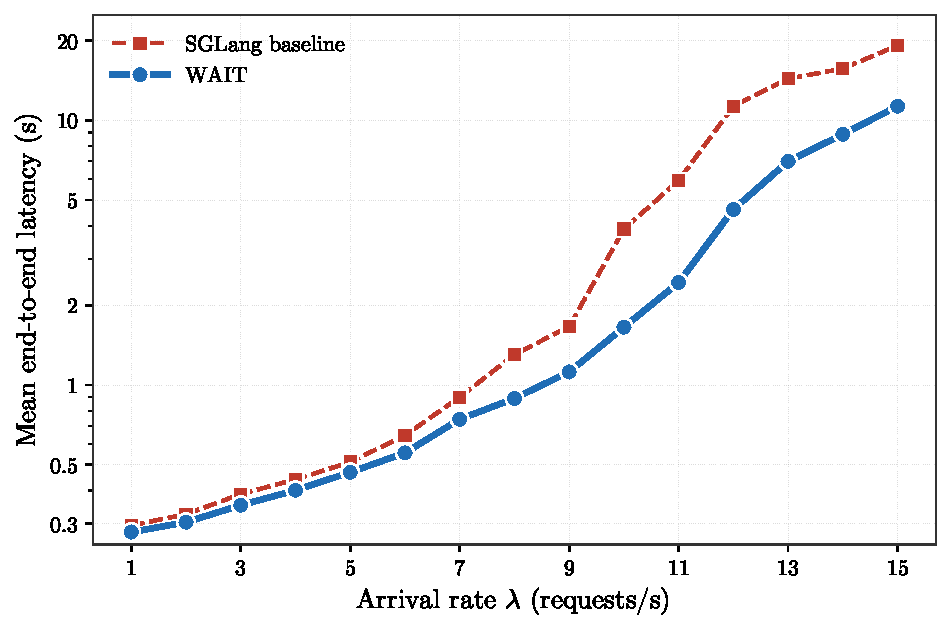
\includegraphics[width=0.65\textwidth]{Experiments_pdf/figure_H_sglang.pdf}
    \caption{Single-type GPU experiment on SGLang~0.5.7 (NVIDIA A100~80\,GB, Llama-2-7B, random prompts with input length $512$ and output length $20$): mean end-to-end latency versus arrival rate. WAIT is compared with the feasible SGLang baseline scheduler configuration used in this experiment and yields a mean latency reduction of $29.7\%$ across the arrival-rate grid.}
    \label{fig:sglang}
\end{figure}

\paragraph{Real dataset on GPU.}
Using the same lmsys-chat-1m workload distribution as Section~\ref{sec:exp_real}, we run paired SGLang experiments with Poisson arrivals at $\lambda \in \{0.1, 0.2, \ldots, 0.7\}$ requests/s and $200$ prompts per rate. The server is restarted before each rate so that the SGLang baseline and Nested WAIT are compared from the same clean GPU state. Nested WAIT uses chunk size $384$ and a rate-specific system-wide batch-size cap $\mathrm{tl}$. For the real-data runs, $\mathrm{tl}$ is distributed over the decode horizon through the listed segment partitions, using the same continuation-based allocation described in Section~\ref{sec:exp_real}. Table~\ref{tab:sglang_realtrace} reports the batch-size caps and decode-stage partitions used in these GPU runs. Figure~\ref{fig:sglang_realtrace} reports mean end-to-end latency in absolute units. Across the tested rates, Nested WAIT has lower latency than the SGLang baseline, with the largest reduction at $\lambda = 0.6$ and an average reduction of $3.6\%$.

\begin{table}[ht]
\centering
\small
\begin{tabularx}{0.82\textwidth}{>{\centering\arraybackslash}p{0.18\textwidth}>{\centering\arraybackslash}p{0.14\textwidth}>{\centering\arraybackslash}X}
\toprule
$\lambda$ (req/s) & $\mathrm{tl}$ & Decode-stage segments \\
\midrule
$0.1$ & $40$  & $[0,175), [175,350), [350,500]$ \\
$0.2$ & $50$  & $[0,210), [210,420), [420,500]$ \\
$0.3$ & $60$  & $[0,200), [200,400), [400,500]$ \\
$0.4$ & $70$  & $[0,175), [175,350), [350,500]$ \\
$0.5$ & $70$  & $[0,200), [200,400), [400,500]$ \\
$0.6$ & $70$  & $[0,175), [175,350), [350,500]$ \\
$0.7$ & $95$  & $[0,250), [250,500]$ \\
\bottomrule
\end{tabularx}
\caption{Nested WAIT parameter settings for the real-data GPU experiment on SGLang~0.5.7 with the lmsys-chat-1m workload distribution, NVIDIA A100~80\,GB, Llama-2-7B, and $200$ prompts per rate. The column $\mathrm{tl}$ gives the system-wide batch-size cap; the decode-stage ranges specify the segment partition over the $500$-token decode horizon. Once these parameters are fixed, the per-stage thresholds are computed by the continuation-based allocation rule in Section~\ref{sec:exp_real}.}
\label{tab:sglang_realtrace}
\end{table}

\begin{figure}[ht]
    \centering
    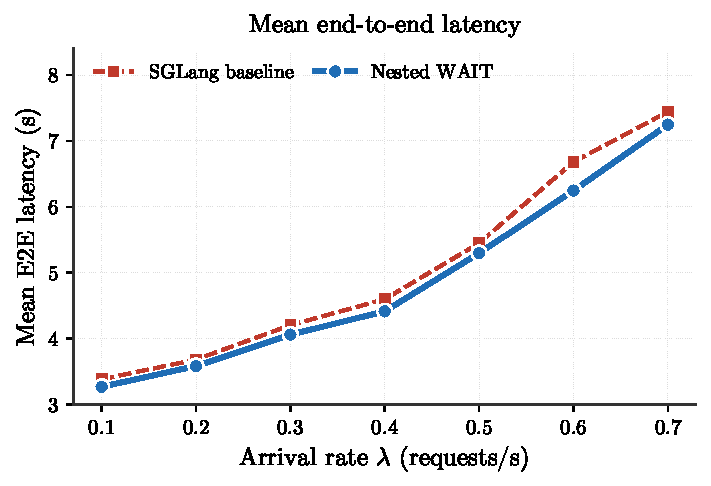
\includegraphics[width=0.58\textwidth]{Experiments_pdf/figure_J_sglang_realtrace.pdf}
    \caption{Real-data GPU experiment on SGLang~0.5.7 with the lmsys-chat-1m workload distribution: mean end-to-end latency versus arrival rate for the SGLang baseline scheduler and Nested WAIT. The Nested WAIT runs use the rate-specific parameter settings in Table~\ref{tab:sglang_realtrace}.}
    \label{fig:sglang_realtrace}
\end{figure}

\subsection{Repeated-run variability}
\label{app:multi_seed}

The main arrival-rate figures in Section~\ref{sec:experiments} report averages over $10$ independent simulation replications at each plotted configuration. To examine sampling variability near the observed transition from near-overloaded to overloaded operation, we additionally repeat the near-transition configurations $20$ times and report the corresponding deviations.

The repeated-run diagnostic preserves the same latency ordering as the main figures across independent arrival draws.

\begin{table}[ht]
\centering
\small
\begin{tabular}{llccc}
\toprule
Workload & $\lambda$ & vLLM (s) & Sarathi (s) & WAIT (s) \\
\midrule
Single-type & $22$ & $18.23\,\pm\,2.74$ & $1.85\,\pm\,0.33$ & $\mathbf{1.03\,\pm\,0.04}$ \\
Single-type & $23$ & $26.78\,\pm\,3.35$ & $5.08\,\pm\,1.72$ & $\mathbf{1.29\,\pm\,0.10}$ \\
Two-type & $22$ & $56.70\,\pm\,2.22$ & $4.06\,\pm\,1.66$ & $\mathbf{2.36\,\pm\,0.57}$ \\
Two-type & $23$ & $80.25\,\pm\,2.37$ & $8.41\,\pm\,1.74$ & $\mathbf{5.66\,\pm\,1.88}$ \\
\bottomrule
\end{tabular}
\caption{Repeated-run reproducibility check near the observed transition from near-overloaded to overloaded operation. Each entry reports mean end-to-end latency together with the sample standard deviation across repeated simulation runs.}
\label{tab:multi_seed}
\end{table}

\subsection{Prefill-decode-disaggregated deployment}
\label{app:pd_disagg}

Production LLM serving increasingly uses a \emph{prefill-decode disaggregation} (PD) architecture, in which prefill and decode are executed by separate services and the KV cache is transferred between them~\citep{patel2024splitwise,zhong2024distserve}. This architecture aligns more closely with the memory-dependent timing model in Section~\ref{sec:model}. Because the decode server no longer mixes prefill and decode work, each iteration processes one token for each active post-prefill job, and the iteration time is driven primarily by active KV-cache usage. The linear iteration-time model in~\eqref{eq:time_consump} is therefore especially appropriate in this setting. The corresponding control decision is how many post-prefill jobs to keep in concurrent decoding; the WAIT threshold implements this decision as an upper bound on the decode-side service population.

We implement this setting in Vidur by using a decode-only request generator: each request enters the simulated decode server after prefill has completed, with post-prefill context length $630$ tokens and decode length $20$ (\texttt{p630d20}). Arrivals follow a Poisson process with $\lambda \in \{100, 150, \ldots, 500\}$ requests/s. In this decode-only setting, Sarathi's chunked-prefill rule no longer changes the scheduling decision, so vLLM's PD scheduler (\texttt{vLLM (PD)}) represents the baseline. Figure~\ref{fig:pd_disagg} reports mean end-to-end decode latency: WAIT improves over vLLM at every rate, with the relative gap ranging from $45\%$ at $\lambda = 100$ to $55\%$ at $\lambda = 500$. Thus, in this tested decode-only setting, the threshold rule improves delay by controlling the decode-side batch composition.

\begin{figure}[ht]
    \centering
    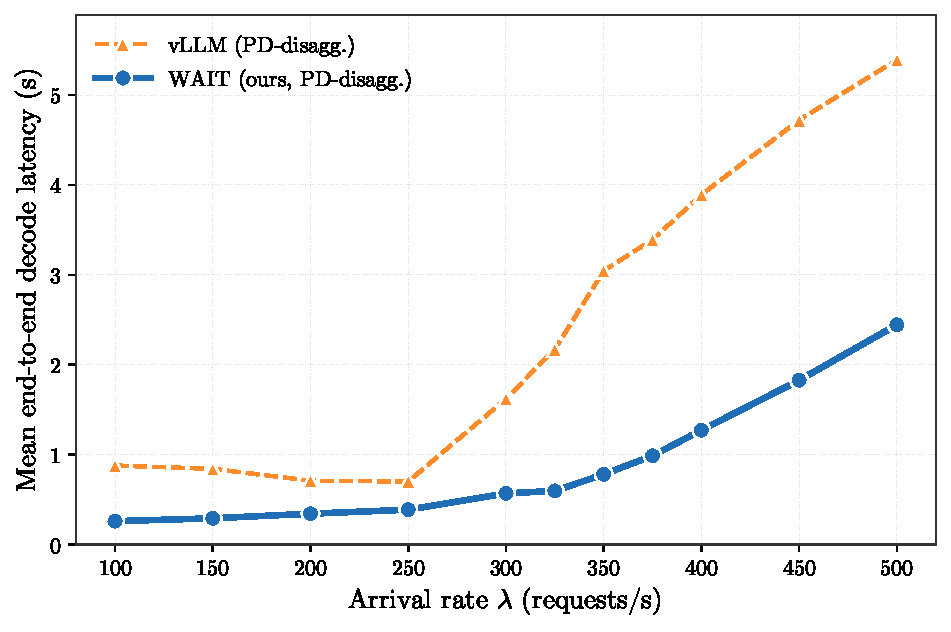
\includegraphics[width=0.65\textwidth]{Experiments_pdf/figure_I_pd_separated.pdf}
    \caption{Prefill-decode-disaggregated deployment (\texttt{p630d20}, decode-only): mean end-to-end decode latency versus arrival rate. WAIT attains between $45\%$ and $55\%$ latency reduction over the vLLM PD baseline across the tested arrival-rate range.}
    \label{fig:pd_disagg}
\end{figure}
